\documentclass[10pt,conference,a4paper]{IEEEtran}
%
\setlength{\marginparwidth}{2cm}
\usepackage{graphicx}
\usepackage{todonotes}
\usepackage{subfigure}
\usepackage{pgfplots}
\usepackage{multirow}
\usepackage{longtable}
\usepackage{booktabs, colortbl, tabularx}
\pgfplotsset{compat=1.6}


\begin{document}
%
\title{NeuroNoC: An Open Reconfigurable Neural Network Prototyping Platform}

\maketitle              % typeset the header of the contribution
%
%\begin{abstract}
%The abstract should briefly summarize the contents of the paper in
%150--250 words.

%\keywords{First keyword  \and Second keyword \and Another keyword.}
%\end{abstract}
%
%
%
\begin{abstract}
\label{sec:abstraction}

\end{abstract}


\begin{IEEEkeywords}
\end{IEEEkeywords}
\section{Introduction}
The growing demand for automated complex intelligent systems leads to dramatic changes in the development and deployment of Artificial Neural Networks (ANN). The capabilities of ANN to map, model and classify nonlinear systems have allowed to incorporate it in various applications in such fields as science, engineering and economics [n]. The development and implementation of ANN has been done mostly in software. However, despite the benefits of software-based ANN such as high level of abstraction (i.e. no need to know the inner workings of ANN for designers), it has severe problems in real-time applications in terms of execution time in contrast to its hardware-based counterparts [e]. In order to address that issue, there have been proposed several hardware adaptations of ANN [f]. Indeed, even though the software implementation offers flexibility, the high-speed operation in real-time applications is only achievable with the hardware-based networks [g].


There has been proposed numerous hardware architectures of ANN, which can be classified into two groups: analog and digital systems. The latter is more popular, since it provides higher accuracy, noise immunity, better scalability, higher flexibility and compatibility. There are three types of digital implementations of hardware-based ANN: field programmable gate array (FPGA) based, digital signal processor (DSP) based and application specific integrated circuit (ASIC) based implementations.  The latter two types of architectures are less suitable for ANN implementation than the first type. DSP based architecture, for instance, is mainly sequential, as a consequence, it lacks to provide parallelism in ANN. ASIC based architectures, on the other hand, does not offer flexibility to reconfigure the ANN by the user [n]. It must be noted that ASIC and DSP can be designed to be highly parallel, however, it is expensive and complicated process to design [e]. FPGA is the best option to implement ANN, since it offers fully parallel and reconfigurable design capabilities.


Reconfigurability of FPGA allows the user to design application specific hardware architecture [g]. FPGA implementations of ANN with a large number of neurons is one of the challenges in hardware-based realizations, since ANN algorithms usually consists of vast amount of multiplication processes and requires higher precision [e]. Hence, on-chip learning is considered to be difficult and useless, as it causes a loss of efficiency in a hardware realization. As a result, off-chip learning is usually chosen when there is no necessity in dynamic learning. Also, the design changes can be made within a few hours, which significantly saves the time and cost of design production. Most of the hardware-based realizations are implemented in such a way that the structure of ANN can be altered through the reprogramming of FPGA [e].


In this paper, we propose the open-source reconfigurable hardware-based realization of ANN, which allows to alter the structure of ANN through the routing of packets in a system. ANN is implemented by the use of mesh topology, which consists of four-way switches with a programming element (PE) connected to it. Each switch with its PE represents a single neuron in ANN. Off-chip learning is chosen in our architecture due to the above-mentioned advantages over on-chip learning. The novelty of the proposed architecture is in the capability of changing the interconnections, weighs and biases on each neuron without explicitly reprogramming the FPGA, but by introducing the ANN configuration packet format, which can be given to the chip the same way as the usual input data packet.  

The main contributions of this work are:
\begin{itemize}
    \item Detailed architecture description of the FPGA-based implementation of ANN
    \item An open-source implementation of ANN targeting the Xillinx Virtex-7
    \item  Characterization of the proposed platform in the terms of resource utilization and performance.
\end{itemize}
 
The rest of the paper is organized as following: Section 2 provides the background, Section 3 discusses the background, Section 4 presents the detailed description of the proposed architecture, Section 5 provides the results f the resource utilization and performance analysis, and Section 6 concludes the paper.

\section{Background and Related Works}



\begin{figure}[t!]
    \centering
    \subfigure[Layered Architecture of Neural Network]
    {
        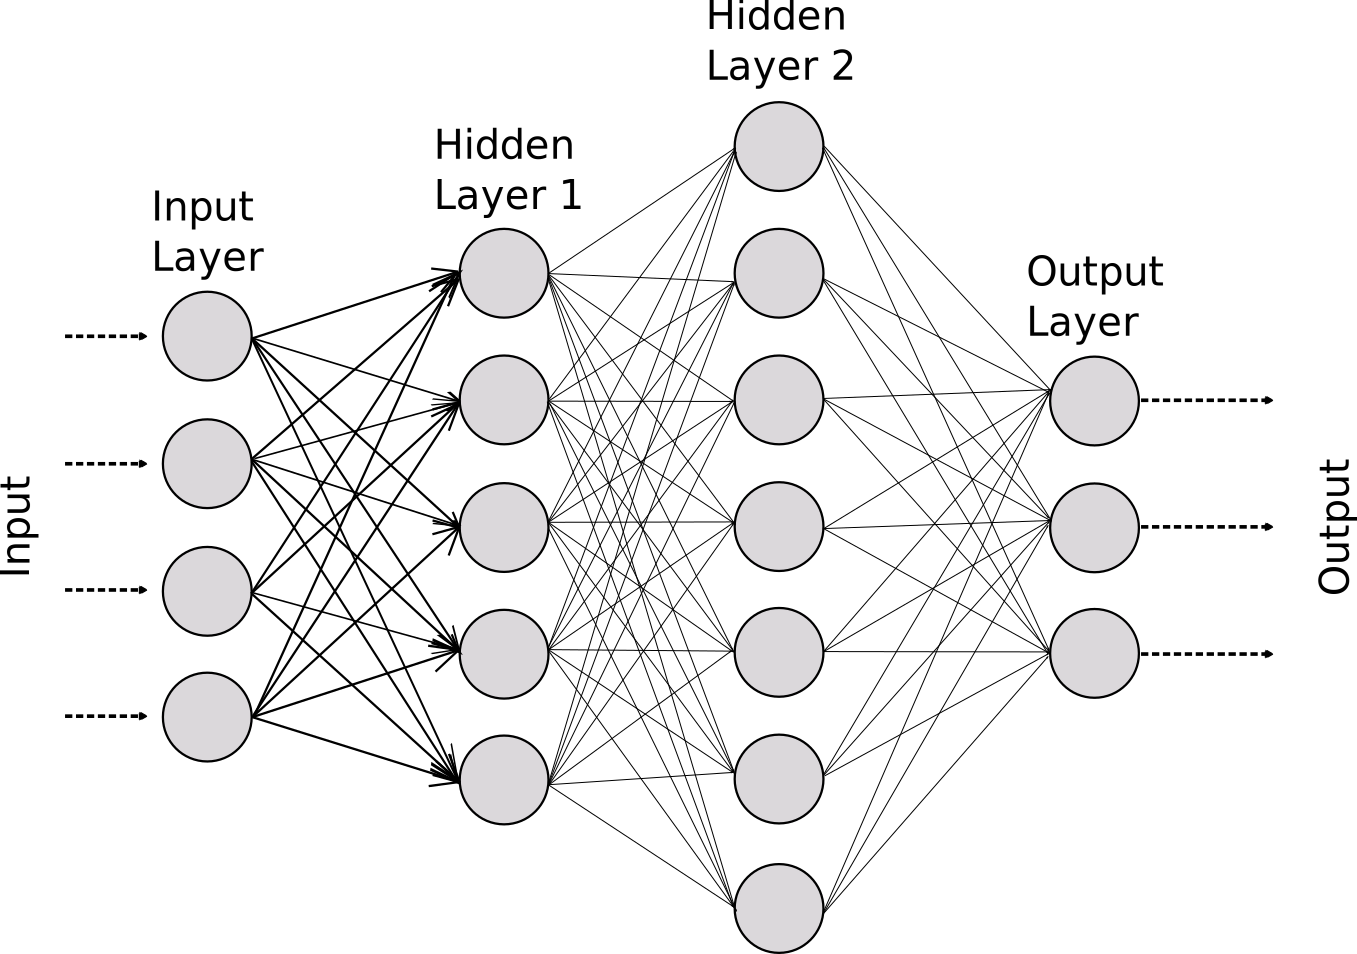
\includegraphics[width = 0.9\columnwidth]{Figures/NeuralNetwork.pdf}
        \label{fig:neuralNetwork}
    }
    \subfigure[A Single Artificial Neuron]
    {
        \label{fig:ann}
        \includegraphics[width = 0.5\columnwidth]{Figures/ANN.pdf}
    }
    \caption{Architecture of a traditional feed-forward neural network and a single artifical neuron}
\end{figure}


~\cite{Furber2013}
Artificial Neural Networks~(ANNs) are inspired and adapted models of biological mammalian brain~\cite{}.
An ANN follows a layered architecture, where each layer is constructed form several neurons as shown in Fig.~\ref{fig:neuralNetwork}. 
In biological neurons, the signal transition takes place between neurons through a structure called \emph{synapse}. 
Each synapse has its own weight, which affects the signal passing though it: the signal is multiplied by the weight of the corresponding synapse. The inputs to the neuron from the synapses are summed up in the neuron and passed further to the activation function. Activation function transforms the input signals to output signals, and its main function is to make decision regarding how the output should behave to certain inputs. Fig. depicts the neuron with the basic operations it performs. 

ANN can consist of many layers, which are classified into three groups: input layer, hidden layer and output layer. One layer can be fully or partially connected to the next layer. Hidden layer can be built from many intermediate layers between input an output. 

\subsection*{Number Representation}

One critical factor in hardware implementation of ANN is the number representation of different data - synapse weights, biases and inputs/outputs of the neurons. Despite its widely usage in software ANNs, floating point arithmetic due to its prohibitively expensive cost is not well suited for hardware ANNs. As a result, the two's complement fixed binary point representation was chosen for data representation as it brings considerable optimization in terms of area usage and speed performance. However, this implies limited precision which is enough for many applications. Nevertheless, with this scheme learning process is accomplished off-chip in software using floating point representation. The conversions from decimal fractions to fixed point binary is done through equation~\ref{equation:dtob}.

\begin{equation}
b_{x}(d_{x})= \lfloor{d_{x}\cdot \frac{2^{n_{x}-1}-1}{2^{i_{x}-1}-2^{-f_{x}}}}\rceil
\label{equation:dtob}
\end{equation}
\begin{equation}
d_{x}(b_{x})= {b_{x}\cdot \frac{2^{i_{x}-1}-2^{-f_{x}}}{2^{n_{x}-1}-1}}
\label{equation:btod}
\end{equation}
Here, $n_{x}$, ${x}$, $f_{x}$ amount to total number of bits, integer bits and fractional bits of the given variable.

The hardware options utilized for machine learning are Central Processing Units (CPU), Graphic
Processing Units (GPU), FPGA and Application-Specific Integrated Circuit (ASIC). 
Each of these options has their own advantages over others. CPUs are extremely flexible in terms of programmability, but they have issues regarding parallelism, cost and heat. 
GPUs have become most widely used hardware option for executing machine learning and deep learning tasks [tpu2]. They are designed to provide high level of parallelism, and thus well suits for the demand of machine and deep learning, where a lot of
matrix multiplications and convolutions are involved.
However, GPUs need to be incorporated with other
chips (e.g. CPU, FPGA) that can rapidly execute NN on it (i.e. inference), since they are more suitable for
training rather than inference. 
FPGAs have recently become popular for machine learning, and companies such as Microsoft and Baidu have invested in FPGAs heavily. 
FPGAs have much less power usage compared to CPUs, and their flexibility offers low latency and high bandwidth. Almost all implementations of ANN on FPGAs use various methods to utilize the reconfigurability of FPGA
hardware. 
According to recent studies, FPGAs have outperformed GPUs in many applications, and it is predicated that they will soon be a better option than GPUs in deep learning [tpu2]. Even though ASICs are the least flexible among other above-mentioned hardware options, they compensate this drawback by offering highest efficiency. ASIC can be designed for both training or inference processes.
There are many examples of ASIC that are designed to meet requirements of machine learning and ANN.
Google’s Tensor Processing Unit (TPU) and IBM’s TrueNorth are the best examples of successful ASIC
deployments for NN purposes. Being originally focused on 8-bit integers for inference tasks, TPUs now
provides floating point precision and can be deployed in training as well [tpu2]. High performance and
power efficiency of TPUs are achieved due to lack of extraneous logic[tpu2]. Hence, unlike other
abovementioned hardware options, TPUs cannot be reprogrammed. IBM’s TrueNorth is a digital chip that
consists of one million spiking-neurons incorporated with 256 million synapses. TrueNorth provides high
efficiency due to spiking-neuron technology, and high scalability as several chips can be tiled in two-
dimensions, as well as flexibility by offering independent configurability of individual neurons and
synapses (noc2). TrueNorth is fabricated using CMOS technology and uses offline learning in NN
purposes (noc2).

\section{Proposed Architecture}

\subsection{Packet Format}:pktformat.  

There are 2 formats of data packets: data packet, and weight, bias, routing table  configuration packet. They are presented in figure~\ref{figure:pktformat}
\begin{figure}[h!]
    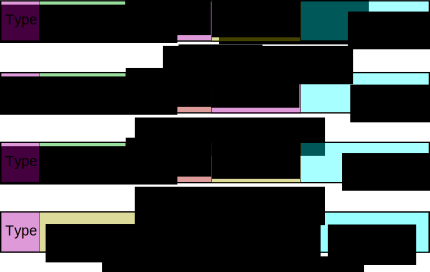
\includegraphics[width=\columnwidth]{Figures/pktformat.pdf}
    \caption{PKTFORMAT} 
    \label{figure:pktformat}
\end{figure}


\subsection{SNC}
The SNC module is a constitutive element underlying the PE design. Since the NOC network is not
designed to ensure the maintenance of correct packet ordering, an imperative design consideration is to
evade out-of-order packet delivery by storing and reassembling the incoming packets. Upon sending
input layer data, sending environment assigns each packet a sequence number which is entered into the
seqNum field. However, it is worth to note that the number being assigned corresponds to the session
number rather than to a single packet i.e a vector comprising n input layer data will be sent in n packets
with same sequence number. After processing the input data, the output packet from PE retains
sequence number of the input packets. The individual units of input layer data are differentiated using
index field, while individual hidden and output layer packets are differentiated using sourceAddress
field.

\begin{figure}
    \centering
    \includegraphics[width =0.4\textwidth]{Figures/overall2.pdf}
    \caption{Caption}
    \label{fig:my_label}
\end{figure}


The figure~\ref{figure:snc} depicts SNC hardware block diagram. The packets arriving from the network
interface are first stored in the hash table (HT) memory. The memory consists of $2^{SEQ\_WIDTH}$ blocks,
where $SEQ\_WIDTH$ amounts to the number of bits in the seqNum field. For the sake of full configurability, for the given NOC of size $S_{NOC}$, each PE can be configured to receive inputs
from up to $S_{NOC}$ terminals. Thus, every block is further divided to contain place for $S_{NOC}$ packets. The packets are mapped into memory through hash function, where

\begin{equation}
hf (seqNum, counter[seqNum]) = concatenate(seqNum, counter[seqNum])
\label{equation:hf}
\end{equation}

Here, the counter[seqNum] embodies the number of packets with the given sequence number that have
arrived to PE and is stored in counter array (CR). After the packet is mapped into appropriate position
within HT, the counter [seqNum] is incremented, so that the next packets with the same sequence
number is stored in the next memory location. The SNC State Machine (SSM) (figure~\ref{figure:sst})
tracks current sequence number and counter to retrieve packets from the HT. The number of inputs
linked to PE is configured using corresponding control packet.

\subsection{MAC}
The computation of the total synaptic input to the neuron constitutes the principal arithmetic operation to be implemented in a hardware design of a neural network. This is done by successive multiplication and addition operators i.e. a series of Multiply-Accumulate (MAC) operations. The reassembled packets from SNC are ushered towards Multiplication (MUL) stage. The weights are associated with the individual input packets through their source address, and these weights are stored in a Weight Table (WT) memory block which is shown in figure~\ref {figure:mac}. The weights can be configured on the run by sending corresponding control packets. The resultant product is accumulated at the Accumulation (ACC) stage. Assuming same format for neuron input and output data, the number of bits to represent weighted sum is

\begin{equation}
N_{s}=\lceil\log_{2}(S_{NOC}\cdot (2^{n_{w}-1})(2^{n_{z}-1})+2^{n_{b}-1}\cdot 2^{f_{z}+f_{w}+f_{b}})\rceil+1
\label{equation:Ns}
\end{equation}

The number of inputs and bias are configured with the same control packets which were used during SNC.  

\subsection{AF}
Implementation of a highly complicated and non-linear activation function, such as a sigmoid function, exploits look-up table (LUT), which may require large amount of memory area depending upon the desirable precision.  If we define $n_{s}$ as the most significant bits of $N_{s}$, increasing the value of $n_{s}$ contributes to the accuracy of the LUT at the expense of memory size. The minimum value at which all the possible output values are present in the LUT is given by

\begin{equation}
n_{s}=i_{s}-\lceil\log_{2}(\frac{d_{z}(1)}{{f}'(0)})\rceil
\label{equation:ns}
\end{equation}

Furthermore, if we consider sigmoid function, most of the entries located too far away from 0 are replicated. With this in mind, it is possible to reduce the size of LUT to store the central interval $[x_{high}, x_{low}]$, in where expressions for $x_{min}$ $x_{max}$ are given by

\begin{equation}
x_{high}=d_{s}(\ln{2^{f_{z}-1}}), x_{low}=-x_{high}
\label{equation:interval}
\end{equation}

and the number of bits to address the LUT is 
$n_{LUT}=\lceil\log_{2}{(x_{high}-x_{low}+1)}\rceil$.
If the computed weighted sum falls within the central interval, then the output is taken from the LUT otherwise the output is assigned either 1 or 0. 


\subsection{NoC}
The figure~\ref{figure:mesh} illustrates the architecture of neural NoC which consists two parts: switches and PE for each of them. The size of NoC can be customized varying $X\_SIZE$ and $Y\_SIZE$,  subsequently number of switches, PE and size of neural network can be configured. For NoC the mesh topology was used, since this topology is convenient for multicast data transmission. Switches connected to each other with four directions: North,South, East, West. Each switch connected to its PE and both of them has unique number depending on their location in the NoC. Each switch and corresponding PE have a unique number depending on their location in the NoC. The sequence starts from left bottom coordinate and increases from left to right and from bottom to top. 

\begin{figure}
    \includegraphics[width=\columnwidth]{Figures/overall3.pdf}
    \caption{MESH} 
    \label{figure:mesh}
\end{figure}

\subsection{Switch}
The inner architecture of one switch is depicted in figure ~\ref{figure:switch_architecture}. Each switch able to send and accept packets from five direction: North, South, East, West and PE. In other words, switch can communicate with upper, lower, right, left neighboring switches and with own PE. Each direction has two FIFO for receiving and transmitting the data. The FIFO was implemented by using IP FIFO generator, therefore, the depth of them can be customized. Switches serve the FIFOs in a queue in a clockwise direction.  Flow control is implemented through AXI-stream control signal as shown if figure.  The $o\_valid$ wires are asserted whenever switch transmits the data for certain direction including PE. Similarly, whenever the data comes from other switches or PE the $i\_valid$ wire of incoming side of the switch is asserted. The switch asserts the $o\_ready$ signal whenever the FIFO has empty slot to accept the data. All FIFOs should hold the data on the bus until data is transmitted to all necessary FIFO. Each switch has registers for routing table, size of total size of NoC rows with 5 bits length. Switch has finite state machine controller, which routes the packet for certain directions depending on the packet type and refreshes the routing table. In one process time one packet can be transmitted to several FIFOs. Switches communicate with each other through FIFOs.  

\begin{figure}
    \includegraphics[width=\columnwidth]{Figures/switch2.pdf}
    \caption{Switch Architecture} 
    \label{figure:switch_architecture}
\end{figure}

\subsection{Routing Packets}
 Switch receives the packet from one FIFO and routes the data for required FIFOs. Finite state machine controller has three main approaches for routing the packets depending on the type of incoming packet.
 For weight and bias configuration packet switch sends the packet using the number of switch in the NoC. Depending on the number of destination switch, the present switch can route the packet for four directions. If the destination switch is located to the above, below, to the left or the right, it sends to North,South, East, West FIFOs respectively. Once the packet came to the predefined switch, instantly it will be sent to the PE FIFO corresponding to that switch for configuring the weight and bias.   
For routing table configuration packets switches behave the same as for weight and bias configuration oriented switches. The one difference is, when the packet came to the destination switch, it will refresh one slot of routing table and switch will serve next FIFO. 

While previous packets can be sent only for one direction(unicast) from one switch, the data packets can be replicated and sent for all direction including PE in one process time (multicast). It was achieved by the logic of routing table. Each switch has routing table, which must be configured before usage. The rows in routing table is equal to the total amount of switches in NoC. The actual meaning of rows in routing table is address of source switch. Whenever data packet comes, switch checks the source provider address of this packet and takes the row, which number is equal to source address. Each row has 5 bits for the decision to sending the packet for certain direction.  Each bit corresponds to 5 directions: North, South, East, West and PE. If the bit is equal to 1 then the incoming packet must be sent to corresponding direction,conversely, if bit is equal to 0 then the packet must not be sent to that direction. The routing table configuration directly depends on the neural network model and configuration packets must be created manually or using other software. For reliability of data in multicasted transmission, switch waits until the data is sent for all necessary direction, only after that it checks next FIFO. For implementation of packet routing the finite state machine principle was used and it is shown in figure ~\ref{figure:fsm}.



\section{Results and Discussion}


\begin{figure}
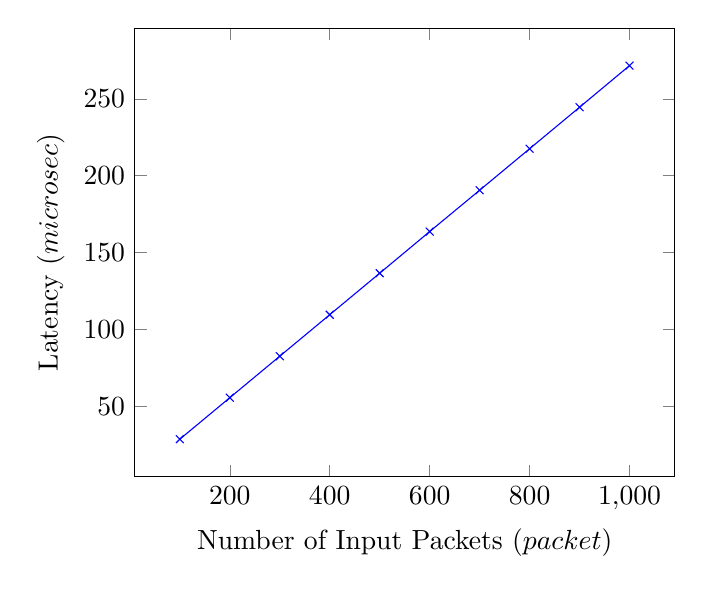
\begin{tikzpicture}
	\begin{axis}[
		xlabel=Number of Input Packets $(packet)$,
		ylabel=Latency $(microsec)$]
	\addplot[color=blue,mark=x] coordinates {
		(100,28.5)
		(200,55.5)
		(300,82.5)
		(400,109.5)
		(500,136.5)
		(600,163.6)
		(700,190.5)
		(800,217.5)
		(900,244.5)
		(1000,271.6)
	};
	\end{axis}
\end{tikzpicture}
\caption{Relationship between latency and the number of input packets} \label{fig:plot1}
\end{figure}


\begin{figure}
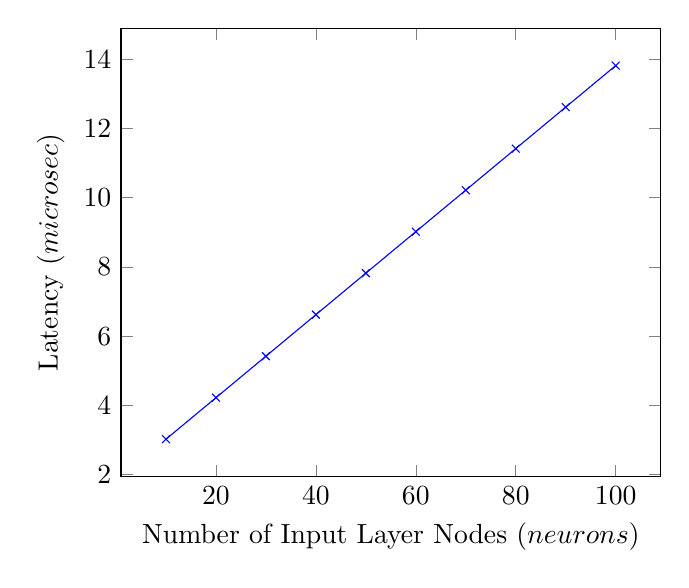
\begin{tikzpicture}
	\begin{axis}[
		xlabel=Number of Input Layer Nodes $(neurons)$,
		ylabel=Latency $(microsec)$]
	\addplot[color=blue,mark=x] coordinates {
		(10,3.02)
		(20,4.22)
		(30,5.42)
		(40,6.62)
		(50,7.82)
		(60,9.02)
		(70,10.22)
		(80,11.42)
		(90,12.62)
		(100,13.82)
	};
	\end{axis}
\end{tikzpicture}
\caption{Relationship between latency and the number of nodes in the input layer} \label{fig:plot1}
\end{figure}

\section{Conclusion and Future Works}






%\bibliographystyle{IEEEtran}
%\bibliography{arc} 
\end{document}
